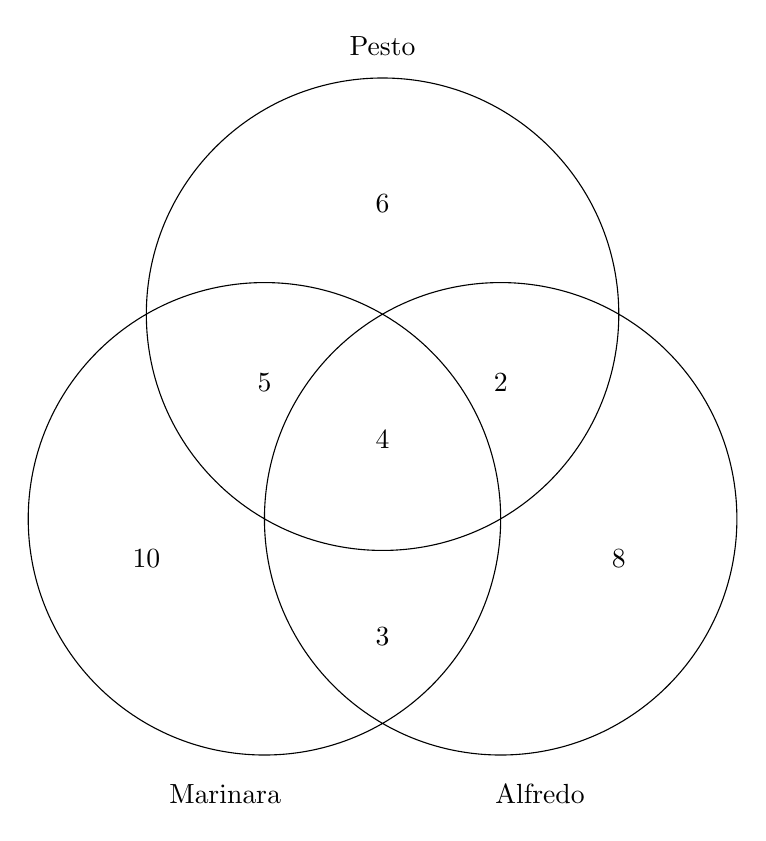
\begin{tikzpicture}
\draw(-1.5,0)circle(3)++(60:3)circle(3)++(300:3)circle(3);
\draw(-3,-.5)node{$10$}(0,1)node{$4$}(3,-.5)node{$8$}(0,4)node{$6$};
\draw(0,-1.5)node{$3$};
\draw(-2.5,0)++(60:2)node{$5$}++(3,0)node{$2$};
\draw(-2,-3.5)node{Marinara}(2,-3.5)node{Alfredo}(0,6)node{Pesto};
\end{tikzpicture}

Out of $60$ people surveyed, $17$ like the pesto sauce, $17$ like the alfredo sauce, and $22$ like the marinara sauce.  The results are shown in the diagram.  How many people surveyed did not like any of the three sauces?



\ifsat
	\begin{enumerate}[label=\Alph*)]
		\item $1$
		\item $16$
		\item $22$%
		\item $36$
	\end{enumerate}
\else
\fi

\ifacteven
	\begin{enumerate}[label=\textbf{\Alph*.},itemsep=\fill,align=left]
		\setcounter{enumii}{5}
		\item $1$
		\item $14$
		\item $16$
		\addtocounter{enumii}{1}
		\item $22$%
		\item $36$
	\end{enumerate}
\else
\fi

\ifactodd
	\begin{enumerate}[label=\textbf{\Alph*.},itemsep=\fill,align=left]
		\item $1$
		\item $14$
		\item $16$
		\item $22$%
		\item $36$
	\end{enumerate}
\else
\fi

\ifgridin
 $22$%
		
\else
\fi

